\documentclass[../resumosRCOM.tex]{subfiles}
 
\begin{document} 
\section{The Data Link Layer}
\subsection{Data Link layer functions and services}
\subsubsection{Main functions}
\begin{itemize}
    \item Provide service interface to the network layer.
    \item Eliminate/reduce transmission errors.
    \item Regulate data flow: Slow receivers not swamped by fast senders.
\end{itemize}

\subsubsection{Services provided}
\paragraph{}
\textbf{Principal service: }Transfer data from the network layer on the 
source machine to the network layer on the destination machine.
\paragraph{}
The actual services that are offered vary from protocol to protocol. 
Three reasonable possibilities that we will consider in turn are:
\begin{itemize}
    \item \textbf{Unacknowledged connectionless service: }
    \begin{itemize}
        \item No logical connection is established beforehand or released
        \item Source machine sends independent frames without having 
        the destination machine acknowledge them. 
        afterwards.
        \item If a frame is lost due to noise on the line, no attempt 
        is made to detector recover from that loss.
        \item Appropriate when the error rate is very low and for 
        real-time traffic.
    \end{itemize}
    
    \item \textbf{Acknowledged connectionless service: }
    \begin{itemize}
        \item No logical connections used.
        \item Each frame sent is individually acknowledged so that the 
        sender knows whether a frame has arrived correctly or been lost.
        \item If it has not arrived within a specified time interval, 
        it can be sent again.
        \item This service is useful over unreliable channels, 
        such as wireless systems.(i.e. Wi-Fi).
    \end{itemize}
    
    \item \textbf{Acknowledged connection-oriented service: }
    \begin{itemize}
        \item The source and destination machines establish a connection 
        before any data are transferred.
        \item Each frame is numbered, and the data link layer guarantees 
        that each frame sent is indeed received.
        \item it guarantees that each frame is received exactly once and 
        that all frames are received in the right order.
        \item Appropriate over long, unreliable links (i.e. satellite channel,
         long-distance telephone circuit). If acknowledged connectionless 
         service were used, lost acknowledgements could cause a frame to be 
         sent and received several times.
        \item Divided in 3 phases:
        \begin{itemize}
            \item \textbf{First phase: }The connection is established by having
             both sides initialize variables and counters needed to keep track of
             which frames have been received and which ones have not.
             \item \textbf{Second phase: } One or more frames are actually transmitted.
             \item \textbf{Third phase: } The connection is released, freeing
            up the variables, buffers, and other resources used to maintain 
            the connection.
        \end{itemize}
    \end{itemize}
\end{itemize}

\paragraph{}
Providing acknowledgements in the data link layer is just an optimization, 
never a requirement. The network layer can always send a packet and wait 
for it to be acknowledged by its peer on the remote machine. 
This strategy,however, can be inefficient. Links usually have a strict maximum
frame length imposed by the hardware, and known propagation delays. 
The network layer does not know these parameters. 
It might send a large packet that is broken up into 10 frames, of which 
2 are lost on average. If individual frames are acknowledged and
retransmitted, then errors can be corrected more directly and more quickly.
On reliable channels, such as fiber, the overhead of a heavyweight data link 
protocol may be unnecessary, but on (inherently unreliable) wireless channels 
it is well worth the cost.

\subsection{Framing}
\paragraph{}
The physical layer accepts and sends a raw bit stream. 
If the channel is noisy the physical layer will add some 
redundancy to its signals to reduce the bit error rate to a tolerable level. 
However, the bit stream received by the data link layer is not guaranteed to 
be error free. It is up to the data link layer to detect and correct errors.
\paragraph{}
The approach is for the data link layer to break up the bit stream into
discrete frames, compute a short token called a checksum for each frame, 
and include the checksum in the frame when it is transmitted.
When a frame arrives at the destination,the checksum is recomputed. 
If it is different from the one contained in the frame, the data link layer
knows that an error has occurred and takes steps to deal with it.
\paragraph{}
A good design must make it easy for a receiver to find the start of new frames
while using little of the channel bandwidth. We will look at three methods:

\subsubsection{Byte count}
\paragraph{}
Uses a field in the header to specify the number of bytes in the 
frame. When the data link layer at the destination sees the byte count,
it knows how many bytes follow and hence where the end of the frame is.

\paragraph{}
Issues
\begin{itemize}
    \item The count can be garbled by a transmission error.     
    \item A single bit flip, may trigger the destination to get
    out of synchronization. 
    \item If an out-of-sync occurs it is unable to locate the correct
    start of the next frame.
\end{itemize}

\begin{figure}[h]
    \centering
    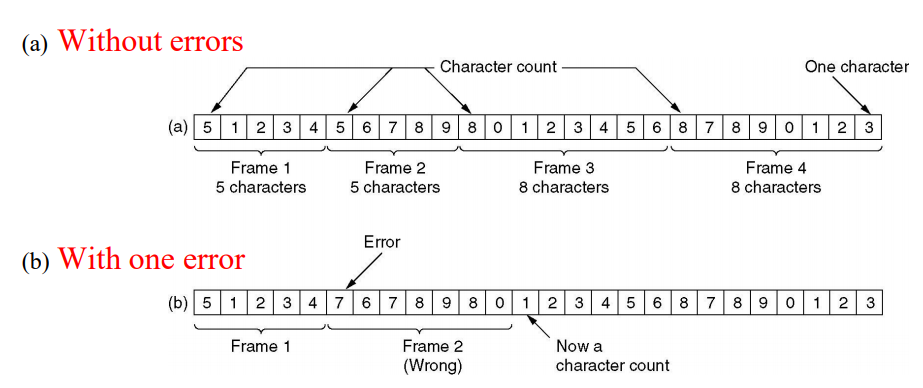
\includegraphics[width=10cm]{byte-count.png}
\end{figure}

This method is rarely used.

\subsubsection{Flag bytes with byte stuffing}
\paragraph{}
This method gets around the problem of resynchronization by having each frame
start and end with special bytes (flag bytes).

\begin{figure}[h]
    \centering
    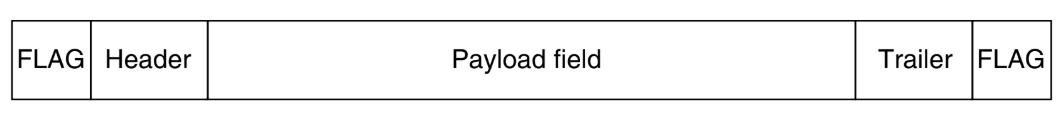
\includegraphics[width=10cm]{byte-stuffing-frame.png}
\end{figure}

\paragraph{}
However, this flag may occur in the middle of the data and induce the receiver
in error by thinking the end of the frame was reached. This issue can be solved
using \textbf{byte stuffing}.

\paragraph{}
\textbf{Byte Stuffing}
\begin{itemize}
    \item Inserting a special escape byte (ESC) before each flag byte in 
    the data.
    \item Makes framing flag bytes distinguishable from the ones in the data.
    \item Escape bytes present in the data also need to be escaped.
\end{itemize}
 
\begin{figure}[h]
    \centering
    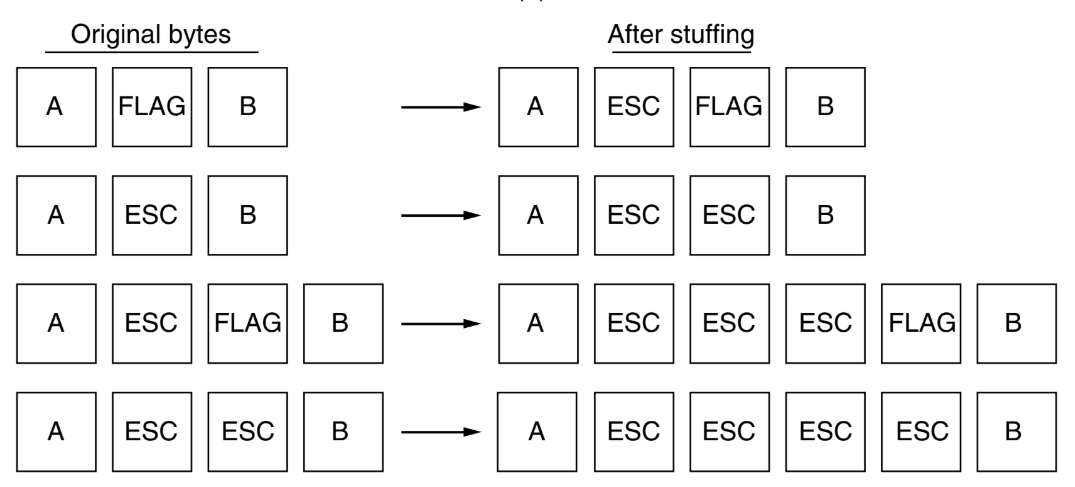
\includegraphics[width=10cm]{byte-stuffing-mechanism.png}
\end{figure}

\subsubsection{Flag bits with bit stuffing}


\subsection{Error detection}
\subsection{Automatic Repeat reQuest (ARQ)}
\subsection{Framing, Error detection and ARQ in common networks}
\subsection{Reliability in the Protocol Stack}

\end{document}